\label{sec:background:preface}

In \cref{ch:introduction}, we defined a common set of (artificial) intelligence-based cloud services that we label \glsplx{cis}. Specifically, we scope the primary body of this study's work on \glsplx{cvcis} (e.g., Google Cloud Vision \citep{GoogleCloud:Home}, AWS Rekognition \citep{AWS:Home}, Azure Computer Vision \citep{Azure:Home}, Watson Visual Recognition \citep{IBM:Home} etc.). We claim developers have a distinctly deterministic mindset ($2+2$ \textit{always}  equals 4) whereas a \gls{cis}'s `intelligence' component (a black box) may return probabilistic results ($2+2$ \textit{might} equal 4 \textit{with a confidence of} 95\%). Thus, there is a mindset mismatch between probabilistic results (from the \gls{api} provider) and results interpreted with certainty (from the \gls{api} consumer).

What affect does this mindset mismatch have on the developer's approach towards building probabilistic software? What can we learn from common software engineering practices (e.g., \citep{Pressman:2005vf,Sommerville:2011uc}) that apply to resolve this mismatch and thereby improve quality, such as \gls{vv}? Chiefly, we anchor this question around three lenses of software engineering: creating a \gls{cis}, using a \gls{cis}, and the nature of \glspl{cis} themselves.

Our chief concern lies with interaction and integration between \gls{cis} providers and consumers, the nature of applications built using a \gls{cis}, and the impact this has on software quality. We triangulate this around three pillars, which we diagrammatically represent in \cref{fig:background:preface:cis-mindset-clash-pillars}.
 
\begin{enumerate}[label=\textbf{(\arabic*})]
\item \textbf{The development of the \gls{cis}.} We investigate the internal quality attributes of creating a \gls{cis} from the \gls{cis} \textit{provider's} perspective. That is, we ask if existing verification techniques are sufficient enough to ensure that the \gls{cis} being developed actually satisfies the \gls{cis} consumer's needs and if the internal perspective of creating the system with a non-deterministic mindset clashes with the outside perspective (i.e., pillar 2).
\item \textbf{The usage of the \gls{cis}.} We investigate the external quality attributes of using a \gls{cis} from the \gls{cis} \textit{consumer's} perspective. That is, we ask if existing validation techniques are sufficient enough to ensure that the end-users can actually use a \gls{cis} to build their software in the ways they expect the \gls{cis} to work.
\item \textbf{The nature of a \gls{cis}.} We investigate what standard software engineering practices apply when developing non-deterministic systems. That is, we tackle what best practices exist when developing systems that are inherently stochastic and probabilistic, i.e., the `black box' intelligence itself.
\end{enumerate}

\begin{figure}[hbt]
  \centering
  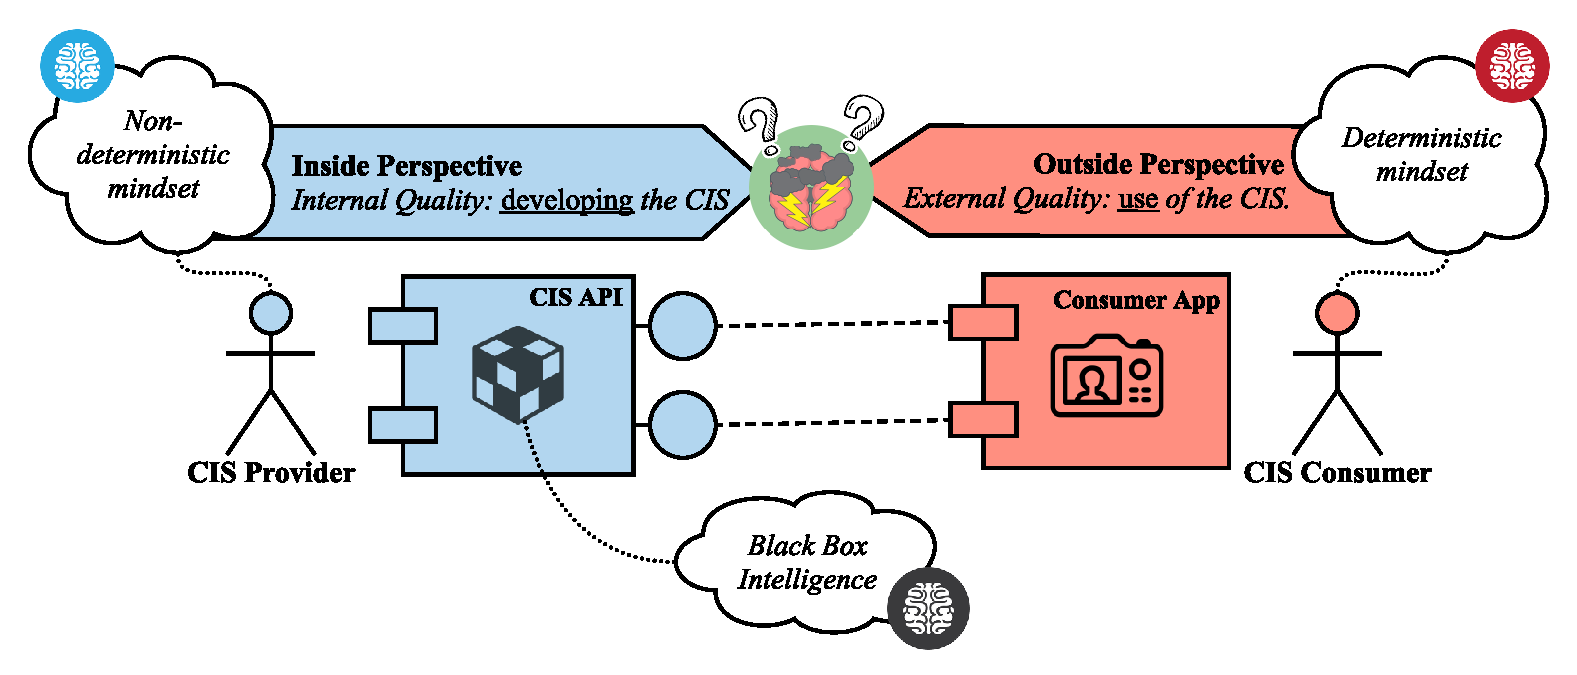
\includegraphics[width=\linewidth]{cis-mindset-clash-pillars}
  \caption[Mindset clashes within the development, use and nature of a CIS]{The three pillars by which we anchor the background: (1) developing a \gls{cis} with a non-deterministic mindset by the \gls{cis} provider; (2) the use of a CIS with a deterministic mindset by the \gls{cis} consumer; (3) the nature of a CIS itself.}
  \label{fig:background:preface:cis-mindset-clash-pillars}
\end{figure}

Does a clash of deterministic consumer mindsets who use a CIS and the non-deterministic provider mindsets who develop them exist? And what impact does this have on the inside and outside perspective? Throughout this chapter, we will review these core principles due to such  mindset mismatch from the anchoring perspective of software quality, particularly around \gls{vv}.
